\documentclass[preprint]{sigplanconf}

% The following \documentclass options may be useful:

% preprint      Remove this option only once the paper is in final form.
% 10pt          To set in 10-point type instead of 9-point.
% 11pt          To set in 11-point type instead of 9-point.
% numbers       To obtain numeric citation style instead of author/year.

\usepackage{amsmath}
\usepackage[pdftex]{graphicx}
\usepackage{float}
\graphicspath{{images/}}

\newcommand{\cL}{{\cal L}}

\begin{document}

\special{papersize=8.5in,11in}
\setlength{\pdfpageheight}{\paperheight}
\setlength{\pdfpagewidth}{\paperwidth}

\conferenceinfo{CONF 'yy}{Month d--d, 20yy, City, ST, Country}
\copyrightyear{20yy}
\copyrightdata{978-1-nnnn-nnnn-n/yy/mm}
\copyrightdoi{nnnnnnn.nnnnnnn}

% Uncomment the publication rights you want to use.
%\publicationrights{transferred}
%\publicationrights{licensed}     % this is the default
%\publicationrights{author-pays}

\titlebanner{banner above paper title}        % These are ignored unless
\preprintfooter{short description of paper}   % 'preprint' option specified.

\title{High-Performance Persistent Graphs}
\subtitle{}

\authorinfo{John Moody}
           {Colorado College '16}
           {john.moody@coloradocollege.edu}
\authorinfo{Benjamin Ylvisaker}
           {Assistant Professor, Colorado College}
           {ben.ylvisaker@coloradocollege.edu}

\maketitle

%should there be some kind of general comment about the current state of persistent data structures, either here or in the introduction?

\begin{abstract}
In the world of persistent data structures, there exist few high performance graph libraries.
We propose in this paper a C library which stores an application-controlled persistent graph in a structure derived from a hash array mapped trie, using chunking and lazy copying to conserve memory and increase performance.
We achieve -some stuff about time complexity that I haven't figured out yet and I have no results help-.
\end{abstract}

\category{CR-number}{subcategory}{third-level}

\keywords
persistent data structures, graphs, hash array mapped trie

\section{Introduction}

A graph is defined as a structure containing some number of nodes and some number of edges, which connect nodes together.
The graph is a data structure with wide-ranging applications, from computational graphs to databases, networking and pathfinding.
To get information about nodes or edges in a graph within a program we typically use an array or some manner of key-value store.
The value associated with a node is usually a list of adjacent nodes, which are either predecessors to that node or antecedents.
We will explore what it means for a graph to be stored in a persistent way, and then propose a structure with strong performance characteristics for various operations and optimized use of memory.

\subsection{Persistence}
What does it mean for data to be stored in a persistent way?
A piece of data is persistent if it does not change.
Consider a linked list in memory, Jeff:
\begin{figure}[H]
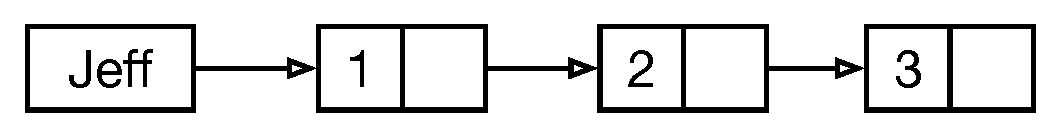
\includegraphics[scale=.35]{linkedlist}
\centering
\end{figure}
There are a number of ways to make an edit to this structure.
If we wanted to change the frontal value of Jeff from 1 to 5, and we do not need the original any longer, we may simply change it:
\begin{figure}[H]
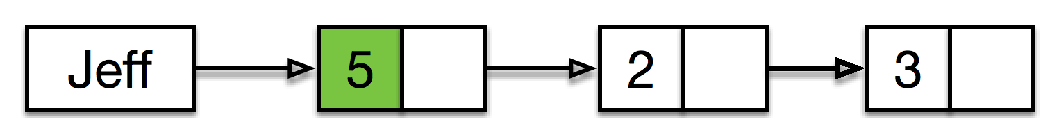
\includegraphics[scale=.35]{linkedlist2}
\centering
\end{figure}
If we want this notion of persistence to apply to Jeff, however, Jeff cannot change.
Instead, we need to come up with a way to change the front value of Jeff to 5 while keeping the original version of Jeff with 1 at the front intact.
Enter "Jeff'":
\begin{figure}[H]
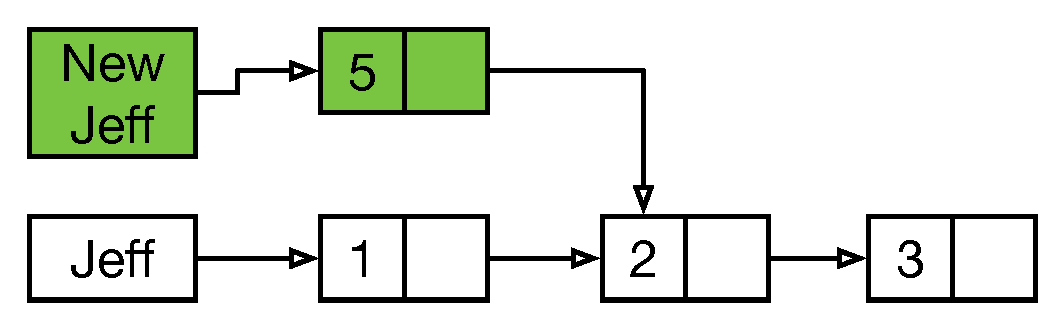
\includegraphics[scale=.35]{linkedlist3}
\centering
\end{figure}
Jeff, we notice, has not changed.
Jeff' preserves the parts of Jeff's structure that they have in common.
Persistent data structures, then, refer to structures like Jeff and Jeff', which, after being created, will always remain the same.

\subsubsection{Trees and Reference Counting}
Let us now consider an example using a simple binary search tree, where we have D, and a separate copy D':
\begin{figure}[H]
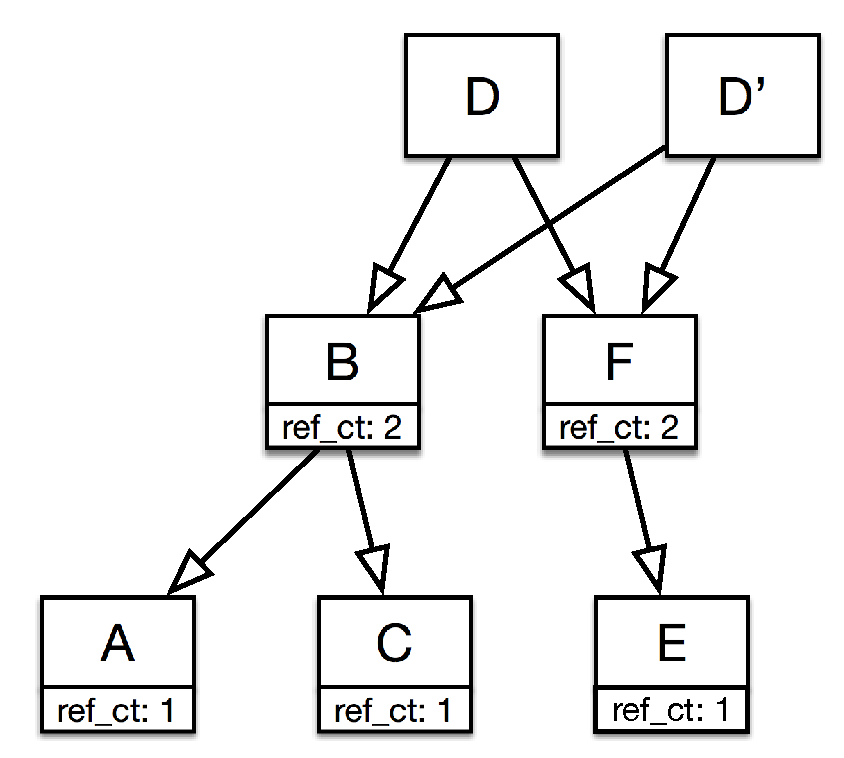
\includegraphics[scale=.43]{treefig}
\centering
\end{figure}
For us to be able to make edits to D' without changing D, we must introduce the concept of reference counting.
A reference count keeps track of how many objects point to a given node.
Here, since B and F have reference counts greater than one, we know that we can't modify those nodes without changing another version of the data structure.
Therefore, when we insert G into D', we will copy any nodes that have reference counts greater than one and adjust the tree as necessary:
\begin{figure}[H]
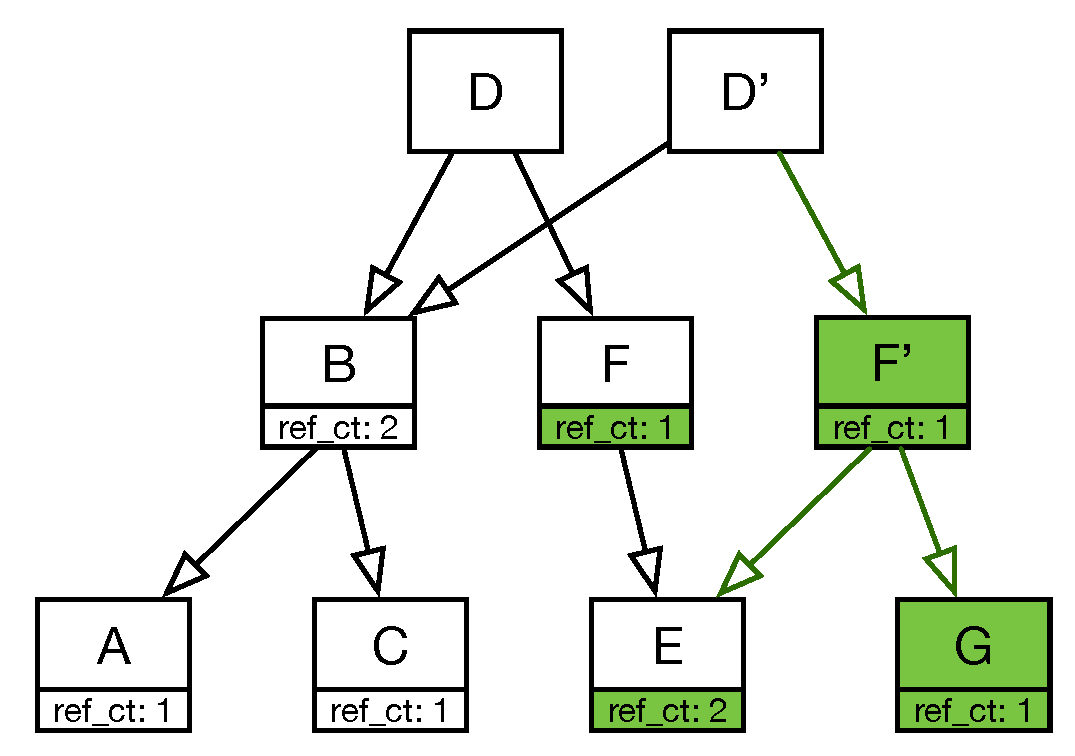
\includegraphics[scale=.43]{treefig2}
\centering
\end{figure}
\subsection{Tries}
How do we represent a graph persistently? We know that whatever structure we use, if we want to efficiently store memory between versions, needs to have elements of tree-like structure, with pointers between discrete parts.
A simple binary search tree is possible, and is used for some persistent graph libraries.
However, the use of a binary search tree introduces significant memory inefficiency.
If a node can only point to two other nodes, trees become very deep very quickly, which means lookups become costly.
Rather, our paper discusses the use of a wide-fanout key-mapped trie, a derivative of the hash array mapped trie (Bagwell, 2000).
Our structure has the following characteristics:
\begin{itemize}
\item The library performs no hashing. Rather, the library assumes a value has a unique key or ID.
\item Values are stored only in leaves.
\item Wide fanout, to minimize tree depth.
\item Array compression, with bitmaps to indicate non-null positions.
\item Values are stored in their parent nodes.
\item Nodes without children are combined with their parents, to reduce the number of pointers.
\end{itemize}
The chunking together of nodes without children with their parents means that nodes are effectively stored by the first unique bits of their key rather than the entire key itself.
To understand how this works, consider a hypothetical insert with keys of length 8, and 4-bit fanout among nodes, of a value with the key 11000110.
Since our fanout is 4 bits, we will consider two bits of the key at a time in determining which branch of the trie to pursue.
\begin{figure}[H]
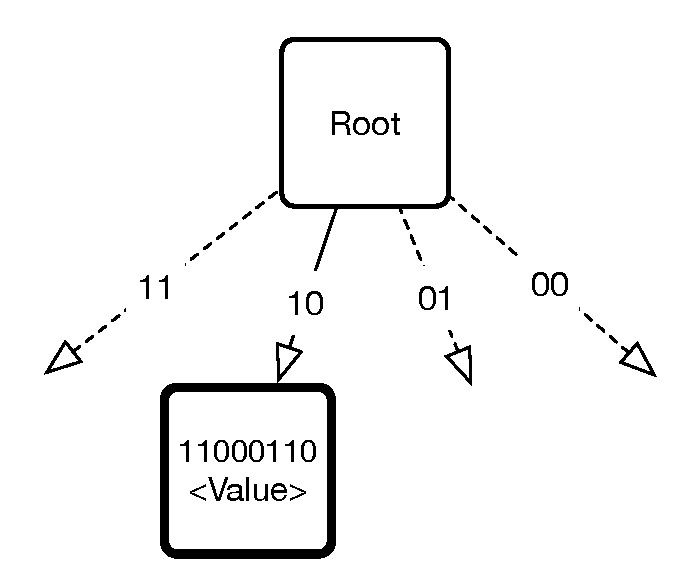
\includegraphics[scale=.5]{trie1}
\centering
\end{figure}
Here, we could create nodes that span the entire depth of the tree to insert the value, but since we would chunk these nodes together later, we will simply store the node by the first section of the key that is unique in the entire set of keys.
Since the root node is empty, we can store the value directly in the first branch.
Since there are no other keys that begin with 10 in the set of keys, we don't need to create an interstitial node.
Inserting a node with a key that also begins with 10 results in the following adjustments:
\begin{figure}[H]
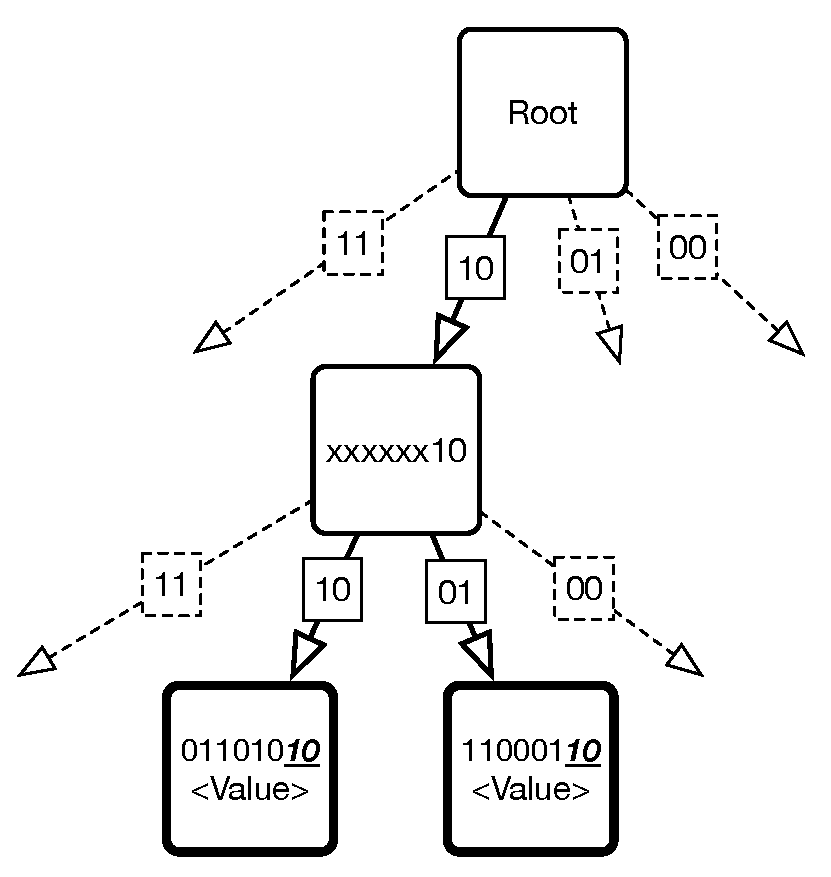
\includegraphics[scale=.5]{trie2}
\centering
\end{figure}
Further, since all values are stored in the leaves of the tree, we will actually store the bolded values in arrays at the tail end of each parent node. Hence, our current trie will actually appear like this in memory:
\begin{figure}[H]
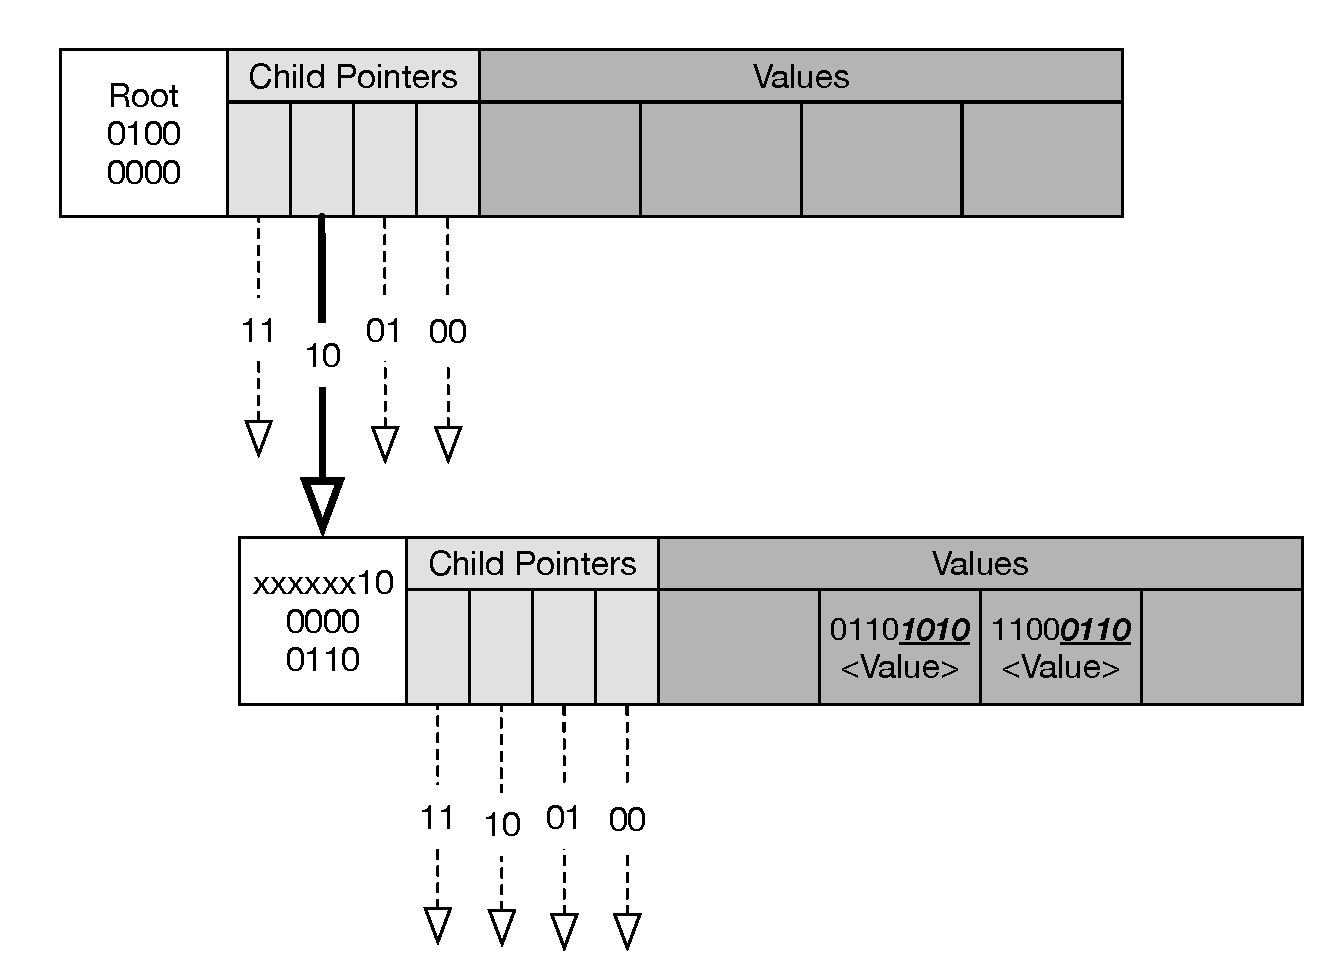
\includegraphics[scale=.4]{trie2actual}
\centering
\end{figure}
Storing these pointers and values in arrays seems to indicate that, for nodes with low populations, we waste a lot of space on empty array slots.
We compensate for this with an array compression scheme borrowed from the hash array mapped trie.
In this scheme, the actual arrays that store pointers and values are dense and dynamically sized.
Each node stores two bitmaps that store data about which spots in our hypothetically complete array are occupied. 
If we want to access a value or pointer at a particular position, we will perform some bitwise arithmetic to determine in which dense array slot our desired value lies.
To illustrate an example, let us consider a bitmap 12 bits in length, which tells us about an array with seven values, 011011101010.
For ease of comprehension, the array will be reversed so that the least significant bits of the bitmap correspond to the lowest indices in the array:
\begin{figure}[H]
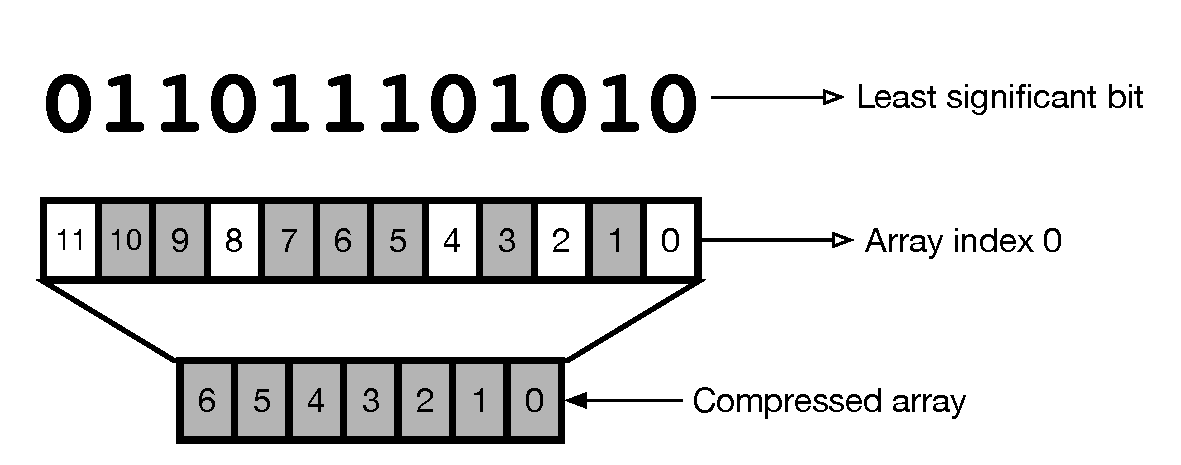
\includegraphics[scale=.5]{bitmask}
\centering
\end{figure}
The bitmap indicates that the keys 2, 4, 6, 7, 8, 10, and 11 are currently occupied by values.
Let's imagine the key we want to use for insertion or lookup is 9.
This means we want to check the 8th index of the bitmap. To verify whether this spot is empty, we will simply bitwise AND together the bitmask and a number whose 8 least significant bits are 1s.
The number of 1s in the result how many spots are occupied in the dense array prior to the one we want to insert into (or, in other words, the index of our desired spot).
We will simply use our built-in popcount instruction to derive the index we need in our dense array, 5:
\begin{figure}[H]
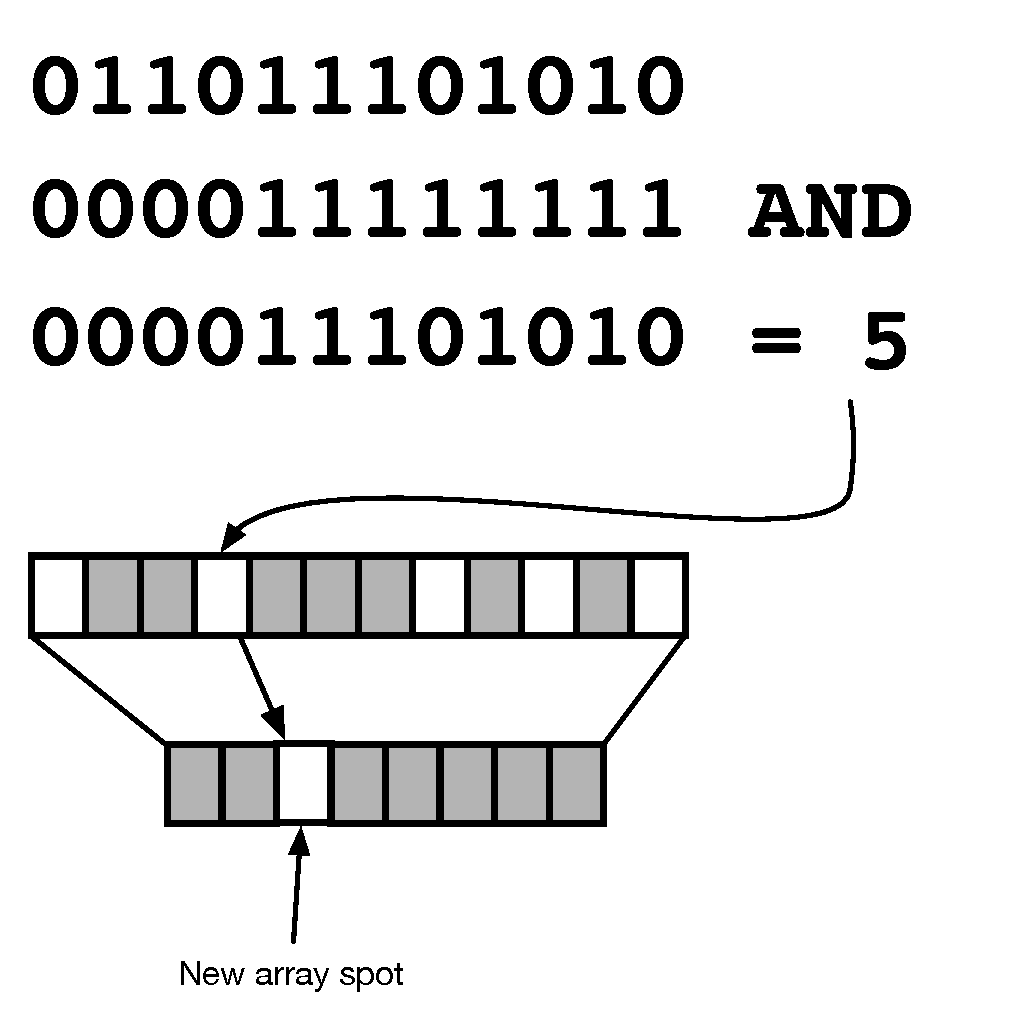
\includegraphics[scale=.5]{bitmask2}
\centering
\end{figure}

\appendix
\section{Appendix Title}

This is the text of the appendix, if you need one.

\acks

Acknowledgments, if needed.

% We recommend abbrvnat bibliography style.

\bibliographystyle{abbrvnat}

% The bibliography should be embedded for final submission.

\begin{thebibliography}{}
\softraggedright

\bibitem[Smith et~al.(2009)Smith, Jones]{smith02}
P. Q. Smith, and X. Y. Jones. ...reference text...

\end{thebibliography}


\end{document}
